\documentclass{article}
\usepackage[utf8]{inputenc}
\usepackage{graphicx}
\graphicspath{ {./image/} }
\title{Stroke Article}
\author{
  {Andor Nagy}
  \and
  {Mikolaj Piotr Kozak}
  \and
  {Marwane Ghalila}
  \and
  {Peter Helle Hartmann}
}

\usepackage[letterpaper,top=2cm,bottom=2cm,left=3cm,right=3cm,marginparwidth=1.75cm]{geometry}
\date{October 2022}

\begin{document}
        \maketitle
        \begin{abstract}
        The causes of stokes can be very difficult to determine, and predicting a stroke is still a hard challenge. Now a days we know a few factors that can be the cause of a stroke but still don't know which one is the most reliable. There is a weak correlation between BMI compared to other factors and no single factor can be used to accurately predict stroke.
        \end{abstract}

\maketitle

\section{Introduction\label{sec:Introduction}}

\subsection{Problem Formulation}
\label{sec:Problem Formulation}
Based on a samples of personal data with features such as age, BMI, average glucose levels we want to find out if a BMI is a strong determinant of stroke.

\subsection{Research Question}
\label{sec:Research Question}
Is BMI a good indicator of stroke risk?
\subsection{Data Set}
\label{sec:Data Set}

For the purpose of this experiment we've relied on 'Stroke Prediction Dataset'. It consists of 5110 records representing individual cases having 11 attributes (gender, age, hyper tension, heart disease, ever married, work type, residence-type, average glucose level, BMI, smoking status, stroke occurrence). There is 0.95 to 0.05 ratio of cases where stroke didn't occur. \\
\begin{center}
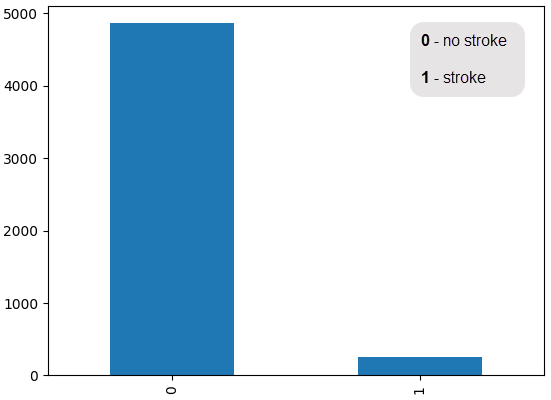
\includegraphics[width=10cm, height=7cm]{image/strokevsNostroke.png}
\end{center}

\section{Methods}
We compare the Spearman's rho correlational coefficient between the various features of the data and stroke events.
We compare the performance of various models trained on a single feature against the same models trained on all features with stroke as the target with AUC as the metric.\\

Methods we used for this project:
Spearman's rho statistical test, Stochastic Gradient Descent Classification, Logistic Regression, Decision Tree Classification, Random Forest Classification,Deep Neural Network

\section{Analysis}
The first test we conducted is a Spearman's Rho statistical test to determine the correlation between BMI and stroke event. The correlational coefficient came out to be 0.05 and the p-value was 0, which would prove the hypothesis but with very weak correlation. We performed the same test on a few other features of interest to see if they might have a stronger correlation than BMI. Average glucose level was shown to be similar, with a coefficient of 0.08, while age proved to have the strongest correlational coefficient of 0.25.

Due to the data having a stroke class imbalance with only 5\% of the samples being positive (i.e. samples with people who had a stroke) accuracy would be a bad metric as any model would easily score at least a 95\% accuracy but would fail miserably at predicting positive cases. Therefore, we decided that AUC would be a more suitable metric. We also decided to perform oversampling on the training data i.e. sampling more fake data to even out the distribution between negative and positive classes. This should improve the performance of certain machine learning models.\cite{class-imba}

Training the various models we noticed that none of the models would perform well when trained only on samples with the BMI feature, with all of them scoring around 0.5 on the AUC metric. In comparison, when training the models on samples with all features, many of them would still perform as badly. Stochastic gradient descent scored 0.76 AUC and logistic regression models scored 0.77.

After that we constructed two deep neural networks, one to be trained on BMI as the only feature and the other to be trained with all features. The networks were constructed with ReLU (Rectified Linear Unit) as the activation function and binary cross-entropy as the loss function. The model trained on BMI only got an AUC score of 0.5567 and of 0.1988 on the test data. The model trained all features got an AUC score of 0.8368 and of 0.1718 on the test data. We can observe a non negligible difference between those results.

\section{Findings}
From the analysis that we conducted we found age had a higher correlational coefficient on stroke than the other features of the data. BMI showed a weak correlation with stroke. We also found that machine learning models trained solely on BMI data would perform no better than random and perform significantly worse than models trained with all features on the data.

\section{Conclusion}
With the results we obtained we can infer that BMI is not a good indicator of stroke risk and where
all the features put together are better at indicating a stoke risk.

\printbibliography
\begin{thebibliography}{1}
\bibitem{class-imba}
Mateusz Buda, Atsuto Maki, and Maciej A Mazurowski. \emph{a document preparation systemA systematic study of the class imbalance problem in convolutional neural networks.} Neural Networks, 106:249–259, 2018.
\end{thebibliography}

\end{document}


